\documentclass[8pt]{beamer}

\usepackage[utf8]{inputenc}
\usepackage[T1]{fontenc}
\usepackage{lmodern}
\usepackage{amsmath}
\usepackage[normalem]{ulem}
\usepackage{tikz}
\usepackage{hyperref}
\usepackage{listings}
\usepackage{color}
\usepackage{fancyvrb}
\usepackage{minted}

\definecolor{links}{HTML}{2A1B81}
\hypersetup{colorlinks,linkcolor=,urlcolor=links}

\usetikzlibrary{shapes,arrows,automata}

\tikzset{
  vertex/.style={
    rectangle,
    rounded corners,
    draw=black, thick,
    text centered
  },
}

\mode<beamer>
{
  \usetheme{Frankfurt}
  \useoutertheme{miniframes}
  \setbeamercovered{transparent}
}

\subject{Talks}

\AtBeginSection[]
{
  \begin{frame}<beamer>{}
    \tableofcontents[currentsection]
  \end{frame}
}

\title[LLVM]{LLVM: Low Level Virtual Machine\\LLVM Intermediate Representation}
\author[Krystian Bacławski]{\href{mailto:cahirwpz@cs.uni.wroc.pl}{Krystian Bacławski}}
\institute{Computer Science Department\\University of Wrocław}
\date{\today}

\begin{document}

\begin{frame}
\titlepage
\end{frame}

\section[Intro]{Introduction}
\subsection*{Ideal world}

\begin{frame}{Stream of instructions}
  \begin{block}{What really does CPU execute?}
    \begin{itemize}
      \item Data flow instructions.
      \item Control flow instructions.
      \item Implicitly organized into Control Flow Graph (CFG).
    \end{itemize}
  \end{block}

  \begin{block}{What is Control Flow Graph?}
    \begin{itemize}
      \item A directed graph.
      \item Each node stores a sequence of data flow instructions \ldots
      \item and finishes with exactly one control flow instruction.
      \item Entry point to each node is labelled.
      \item Control flow instruction include: direct jump, indirect jump,
        function call / return, conditional branch, exception.
      \item Edges are determined by behaviour of the last instruction.
      \item $\forall n \in V. pred(n) \ge 1 \lor succ(n) \ge 1$
    \end{itemize}
  \end{block}
\end{frame}

\begin{frame}{Control Flow Graph terminology}
  \begin{block}{Blocks}
    \begin{description}
      \item[BB] Basic block is a node of CFG.
      \item[Entry block] Has no predecessor (source).
      \item[Exit block] Has no successors (sink).
      \item[EBB] Linear sequence of basic blocks, which can be entered from outside only through one node.
    \end{description}
  \end{block}

  \begin{block}{Edge}
    \begin{description}
      \item[back] goes to predecessor (loop)
      \item[critical] $(a,b) \in E$ is critical if $succ(a) > 1 \land pred(a) > 1$ -- requires splitting. 
      \item[abnormal] "dangling" edge -- jump to address not known at compile-time.
    \end{description}
  \end{block}

  \begin{block}{Dominance relation}
    Consider a control flow graph $G$ with two nodes $v$, $w$, and an entry
    block $s$. \\
    If every path from $s$ to $w$ contains $v$, then $v$ dominates $w$, written
    $v \gg w$.
  \end{block}
\end{frame}

\begin{frame}[fragile=singleslide]{Control Flow Graph examples}
  \begin{columns}[c]
    \column{.33\textwidth}
    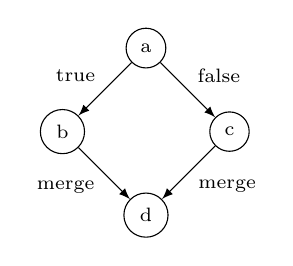
\begin{tikzpicture}[->, font=\scriptsize, >=latex, auto, node distance=1.5cm]
      \tikzstyle{every state}=[circle, draw, minimum size=0.5cm]
      \node[state] (a) {a};
      \node[state] (b) [below left of=a] {b};
      \node[state] (c) [below right of=a] {c};
      \node[state] (d) [below right of=b] {d};
      \path
      (a) edge node[left,yshift=0.5em]{true} (b) 
      (a) edge node[right,yshift=0.5em]{false} (c) 
      (b) edge node[left,yshift=-0.5em]{merge} (d) 
      (c) edge node[right,yshift=-0.5em]{merge} (d);
    \end{tikzpicture}
    \begin{minted}[gobble=6]{c}
      if (a)
        b;
      else
        c;
      d;
    \end{minted}

    \column{.33\textwidth}
    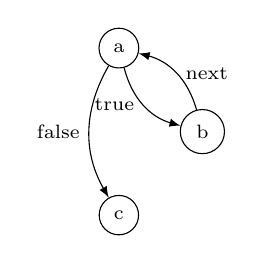
\begin{tikzpicture}[->, font=\scriptsize, >=latex, auto, node distance=1.5cm]
      \tikzstyle{every state}=[circle, draw, minimum size=0.5cm]
      \node[state] (a) {a};
      \node[state] (b) [below right of=a] {b};
      \node[state] (c) [below left of=b] {c};
      \path 
      (a) edge [bend right=30] node[left]{true} (b)
      (b) edge [bend right=30] node[right]{next} (a)
      (a) edge [bend right=30] node[left]{false} (c);
    \end{tikzpicture}
    \begin{minted}[gobble=6]{c}
      while (a)
        b;
      c;
    \end{minted}

    \column{.33\textwidth}
    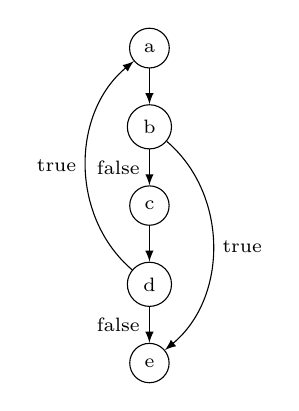
\begin{tikzpicture}[->, font=\scriptsize, >=latex, auto, node distance=1.0cm]
      \tikzstyle{every state}=[circle, draw, minimum size=0.5cm]
      \node[state] (a) {a};
      \node[state] (b) [below of=a] {b};
      \node[state] (c) [below of=b] {c};
      \node[state] (d) [below of=c] {d};
      \node[state] (e) [below of=d] {e};
      \path
      (a) edge (b)
      (b) edge [bend left=50] node[right]{true} (e)
      (b) edge node[left]{false} (c)
      (c) edge (d)
      (d) edge [bend left=50] node[left]{true} (a)
      (d) edge node[left]{false} (e);
    \end{tikzpicture}
    \begin{minted}[gobble=6]{c}
      do
      {
        a;
        if (b)
          break;
        c;
      } while (d);
      e;
    \end{minted}
  \end{columns}
\end{frame}

\begin{frame}[fragile]{SSA form}
  \begin{figure}
    \centering
    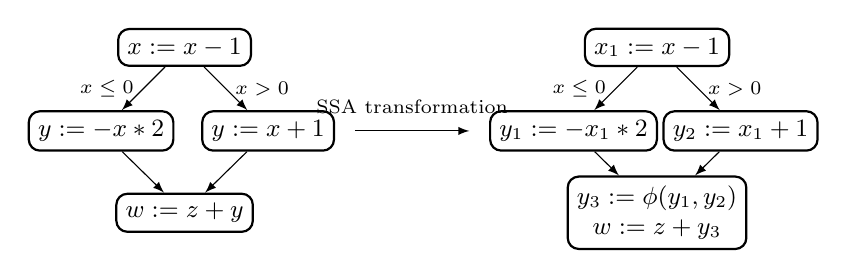
\begin{tikzpicture}[auto,node distance=1.5cm,font=\small]
      \begin{scope}
        \node[vertex] (a) {$x := x - 1$};
        \node[vertex, below left of=a] (b) {$y := -x * 2$};
        \node[vertex, below right of=a] (c) {$y := x + 1$};
        \node[vertex, below of=a,yshift=-0.6cm] (d) {$w := z + y$};
        \path[->,font=\scriptsize,>=latex]
        (a) edge node[left]{$x \leq 0$} (b)
        (a) edge node[right]{$x > 0$} (c)
        (b) edge (d)
        (c) edge (d);
      \end{scope}

      \begin{scope}[xshift=6cm]
        \node[vertex] (a') {$x_1 := x - 1$};
        \node[vertex, below left of=a'] (b') {$y_1 := -x_1 * 2$};
        \node[vertex, below right of=a'] (c') {$y_2 := x_1 + 1$};
        \node[vertex, below of=a',yshift=-0.6cm,align=center]
        (d') {$y_3 := \phi(y_1,y_2)$ \\ $w := z + y_3$};
        \path[->,font=\scriptsize,>=latex]
        (a') edge node[left]{$x \leq 0$} (b')
        (a') edge node[right]{$x > 0$} (c')
        (b') edge (d')
        (c') edge (d');
      \end{scope}

      \draw [->,>=latex,shorten >=2.5mm,shorten <=2.5mm] (c) -- (b')
      node [above=1mm,font=\scriptsize,midway,text centered] {SSA transformation};
    \end{tikzpicture}
    \caption{Example of SSA transformation for simple \texttt{if-then-else} statement.}
  \end{figure}

  \begin{block}{\textit{Static Single Assignment} form properties}
    \begin{itemize}
      \item Variables propagate along edges.
      \item Variables, once assigned, cannot be changed!
      \item $\phi(\ldots)$ operator merges value which flows down from several nodes.
      \item Thanks to immutability better properties for code analysis
        algorithms.
      \item Some optimizations are available almost for free (eg. dead code
        elimination).
    \end{itemize}
  \end{block}
\end{frame}

\begin{frame}{Normalization and lowering.}
  There's well known algorithm to transform code into SSA form (dominance frontiers).

  Lowering looses information.
\end{frame}

\begin{frame}{Optimization levels}
  function level
  IPO
  LTO
\end{frame}

\subsection*{Real world}

\begin{frame}{Processor model}
  \begin{block}{RISC architecture}
    \begin{itemize}
      \item Most instructions have three operands.
      \item Load-store architecture.
      \item Register machine (floating-point, integer).
      \item Finite number of architectural registers (usually 32).
      \item Minimal hardware support for stack.
      \item Few machine types (integers of different width).
      \item Instructions carry information how to interpret data in registers or memory.
      \item Simple conditional jumps (NE, EQ).
    \end{itemize}
  \end{block}

  \begin{block}{ISA vs. microarchitecture}
    \begin{itemize}
      \item \textit{Instruction Set Architecture} is an interface between a compiler and the machine.
      \item Processor is a realization of some microarchitecture.
      \item ISA abstracts how CPU actually executes instructions.
      \item There are many ways to execute same instruction stream correctly!
      \item To generate efficient code you have to understand microarchitecture!
    \end{itemize}
  \end{block}
\end{frame}

\begin{frame}{Memory hierarchy}
  \begin{alertblock}{Problems with DRAM}
    Memories are several hundred times slower than registers. Memory technology
    could not follow up processors for last 30 years! Processors can calculate
    very quickly, but how to feed them with instruction and data at desired
    rate.
  \end{alertblock}

  \begin{block}{Locality}
    Human-written code exposes memory access locality:
    \begin{description}
      \item[temporal] reference same data over and over (variables),
      \item[spatial] reference nearby location (data structures).
    \end{description}
    \vspace{1em}
    How to exploit locality?
    \begin{itemize}
      \item Cache memory -- stores working set, block transfer.
      \item Delayed writing -- write-back policy.
      \item Prefetching and speculation.
    \end{itemize}
    \vspace{1em}
    \textbf{Compilers perform cache-aware optimizations but only w.r.t.
      instruction stream.}
  \end{block}
\end{frame}

\begin{frame}[fragile]{ILP}
  \begin{block}{Instruction Level Parallelism}
    Modern processors are able to "execute" multiple instructions at once -- an
    order of 100 is not uncommon. They can issue several instruction from BB at
    once and can speculate execution of successive BBs.
  \end{block}

  \begin{block}{Hazards}
    Control and data hazards limit ILP and thus processors throughput.
    \begin{description}
      \item[control] conditional branches, indirect jumps, exceptions
      \item[RAW] real dependency (limits data flow)
        \begin{Verbatim}[commandchars=\\\{\}]
          \underline{R2} <- R1 + R3
          R4 <- \underline{R2} + R3
        \end{Verbatim}
      \item[WAR] anti-dependency
        \begin{Verbatim}[commandchars=\\\{\}]
          R4 <- R1 + \underline{R5}
          \underline{R5} <- R1 + R2
        \end{Verbatim}
      \item[WAW] output dependency
        \begin{Verbatim}[commandchars=\\\{\}]
          \underline{R2} <- R4 + R7
          \underline{R2} <- R1 + R3
        \end{Verbatim}
    \end{description}
  \end{block}
\end{frame}

\begin{frame}{ILP exploitation techniques}
  \begin{alertblock}{}
    Many papers about observed ILP. Conclusions not decisive -- advancements in
    compiler and processor technology change assumptions every $n$ years.
  \end{alertblock}

  \begin{block}{Most successful techniques}
    \begin{itemize}
      \item Divide instruction execution into phases -- pipelining.
      \item Analyse data hazards and try to issue several instructions per
        clock cycle.
      \item Allow to execute instructions out of order.
      \item Avoid \textbf{WAR} and \textbf{WAW} with register renaming.
      \item Employ aggressive branch prediction to speculate instruction execution.
    \end{itemize}
  \end{block}

  \begin{alertblock}{}
    Processors effectively perform dynamic analysis on the running code. Having
    extra internal registers they partially undo suboptimal register assignment.
    Fragments of CFG is partially recovered thanks to trace caches.\\
    \vspace{1.0em}
    \textbf{Widely accepted methods of program encoding seems to be highly
      ineffective!}
  \end{alertblock}
\end{frame}

\begin{frame}{Application Binary Interface}
  \begin{block}{Symbols and name mangling}
    \begin{itemize}
      \item A mapping from identifier and object's type into a link-time symbol.
      \item Do we need to encode function's signature into a symbol (due to overloading)?
      \item Any attributes associated with a symbol (visibility, linking, optimization)?
    \end{itemize}
  \end{block}
    
  \begin{block}{Function calling convention}
    \begin{itemize}
      \item Where to put arguments (stack or registers)?
      \item Where the result is available?
      \item How to create activation record?
      \item Which registers need to be saved and restored?
    \end{itemize}
  \end{block}

  \begin{block}{Data and memory organization}
    \begin{itemize}
      \item Which bit is MSB and LSB?
      \item Big-endian or little-endian?
      \item Alignment requirements for words?
      \item Size of machine data types (integer, float, etc.)?
    \end{itemize}
  \end{block}
\end{frame}

\begin{frame}{Linker}
\end{frame}

\begin{frame}{Run-time environment}
\end{frame}

\section[Features]{LLVM features}
\subsection*{LLVM machine model}

\begin{frame}[fragile]{Virtual machine model}
  \begin{block}{Implemented model:}
    \begin{itemize}
      \item Register based machine -- infinite number of virtual registers.
      \item Implicit stack -- no stack management else than variable placement.
      \item Instruction stream in SSA (static single assignment) form.
      \item Strongly typed machine:
        \begin{itemize}
          \item explicit coercions between numeric machine types,
          \item typed pointers!
        \end{itemize}
      \item RISC-like load-store approach to memory access.
      \item Compound (structures) and aggregate types (vectors).
      \item Heavily influenced by \verb+C+ language but versatile enough.
    \end{itemize}
  \end{block}
  
  \begin{block}{Some interesting extra features:}
    \begin{itemize}
      \item Language agnostic exception handling (incl. DWARF2 stack unwinding).
      \item Support for accurate garbage collection.
      \item Atomic memory access for concurrent programming.
    \end{itemize}
  \end{block}
\end{frame}

\begin{frame}[fragile]{Types}
  \begin{block}{Type system of LLVM:}
    \begin{itemize}
      \item Machine oriented!
      \item Types known from C language: integer, floating point, label,
        void, array, function, pointer, structure (but no unions!)
      \item \ldots and LLVM specific: vector (for SIMD), opaque (forward
        declaration).
      \item Most types are first-class. You cannot create a function type.
        However it's valid to create a pointer to function type.
    \end{itemize}
  \end{block}

  \begin{block}{Type notation:}
    \begin{description}
      \item[i1] boolean represented as a single-bit integer
      \item[array] \verb+[ <#elements> x <element type> ]+
      \item[vector] \verb+< <#elements> x <element type> >+
      \item[structure] \verb+type { <type list> }+
    \end{description}
  \end{block}
\end{frame}

\section[Language]{LLVM language}
\subsection*{LLVM IR basics}

\begin{frame}[fragile]{Values}
  \begin{block}{Values:}
    \begin{itemize}
      \item special: \verb+null+, \verb+true+, \verb+false+, \verb+undef+,
        \verb+zeroinitializer+.
      \item notion of being constant.
    \end{itemize}
  \end{block}
\end{frame}

\begin{frame}[fragile]{Instructions}
  \begin{block}{}
    \begin{itemize}
      \item Arithmetic instructions:
        \begin{itemize}
          \item integer: \verb+add+, \verb+sub+, \verb+mul+, \verb+udiv+,
            \verb+sdiv+, \verb+urem+, \verb+srem+, \verb+icmp+
          \item floating-point: \verb+fadd+, \verb+fsub+, \verb+fmul+, \verb+fdiv+,
            \verb+frem+, \verb+fcmp+
        \end{itemize}

      \item Bitwise instructions:
        \begin{itemize}
          \item bit-shift: \verb+shl+, \verb+lshr+, \verb+ashr+
          \item boolean: \verb+and+, \verb+or+, \verb+xor+
        \end{itemize}

      \item Control flow instructions:
        \begin{itemize}
          \item function calls: \verb+invoke+, \verb+call+, \verb+ret+
          \item jumping: \verb+br+, \verb+switch+, \verb+indirectbr+
          \item other: \verb+phi+, \verb+select+
        \end{itemize}

      \item Memory access instructions:
        \begin{itemize}
          \item stack space allocation: \verb+alloca+
          \item generic accessors: \verb+load+, \verb+store+
        \end{itemize}

      \item Compound data access instructions:
        \begin{itemize}
          \item vectors: \verb+extractelement+, \verb+insertelement+, \verb+shufflevector+
          \item aggregates: \verb+extractvalue+, \verb+insertvalue+
          \item other: \verb+getelementptr+
        \end{itemize}

      \item Data conversion instructions:
        \begin{itemize}
          \item integer: \verb+trunc+, \verb+zext+ \verb+sext+
          \item floating-point: \verb+fptrunc+, \verb+fpext+, \verb+fptoui+,
            \verb+fptosi+, \verb+uitofp+, \verb+sitofp+,
          \item pointers: \verb+ptrtoint+, \verb+inttoptr+, \verb+bitcast+
        \end{itemize}
    \end{itemize}
  \end{block}
\end{frame}

\begin{frame}[fragile]{Non-control flow instruction examples}
  \begin{exampleblock}{}
    \begin{minted}[gobble=6,linenos,fontsize=\small]{llvm}
      %r0 = add i32 4, %num                             ; r0 := 4 + %num
      %r1 = fdiv float 11.0, %fp                        ; r1 := %fp / 11.0
      %r2 = or i1 %b1, %b2                              ; r2 := %b1 || %b2
      %r4 = extractelement <4 x i32> %vec, i32 0        ; r4 := %vec[0]
      %r5 = insertvalue {i32, float} %agg, float %v, 1  ; r5 := %agg{[1] = %v}
      %ptr = alloca i32                                 ; {i32 *}
      store i32 3, i32* %ptr                            ; void : *(%ptr) = 3
      %v = load i32* %ptr                               ; i32 : v := *(%ptr)
      %p = icmp eq i32 %n, 0                            ; bool : p := (%n = 0)
      %z = select i1 %p, i8 %x, i8 %y                   ; %z = %p ? %x : %y
    \end{minted}
  \end{exampleblock}

  \begin{block}{Comments:}
    \begin{itemize}
      \item Integer: different signedness and word size possible, overflow
        control.
      \item Floating-point: different word size possible, compliance with
        \verb+IEEE754+.
      \item Boolean calculation for \verb+i1+ type.
      \item \verb+alloca+ is the only instruction dealing with stack.
      \item SSA is performed only for registers, not memory locations.
      \item Choice of type essential for optimization.
    \end{itemize}
  \end{block}
\end{frame}

\begin{frame}[fragile]{Control flow instruction examples}
  \begin{exampleblock}{Infinite loop that counts from 0 on up\ldots}
    \begin{minted}[gobble=6,linenos,fontsize=\small]{llvm}
      LoopHeader:
        ...
        br label %Loop

      Loop:
        %IndVar = phi i32 [ 0, %LoopHeader ], [ %NextIndVar, %Loop ]
        %NextIndVar = add i32 %IndVar, 1
        br label %Loop
    \end{minted}
  \end{exampleblock}

  \begin{block}{First basic control flow graph!}
    \begin{itemize}
      \item $\phi(\ldots)$ syntax: \verb+<result> = phi <type> [<val0>, <label0>], ...+
      \item $\phi(\ldots)$ states:
        \begin{itemize}
          \item how control flow can reach given node?
          \item which value to select depending on previous node?
        \end{itemize}
    \end{itemize}
  \end{block}
\end{frame}

\begin{frame}[fragile]{Call instruction examples}
  \begin{exampleblock}{Function call examples:}
    \begin{minted}[gobble=6,linenos,fontsize=\small]{llvm}
      %retval = call i32 @test(i32 %argc)
      call i32 (i8*, ...)* @printf(i8* %msg, i32 12, i8 42)
      %X = tail call i32 @foo()
      %struct.A = type { i32, i8 }
      %r = call %struct.A @bar()
      %Z = call void @foo() noreturn
    \end{minted}
  \end{exampleblock}

  \begin{block}{Comments:}
    \begin{itemize}
      \item Different calling convention (\verb+fastcc+, \verb+ghc+, \ldots)
      \item \verb+varargs+ functions supported.
      \item Can return compound and aggregate types.
      \item Special attribute for tail-call optimization.
      \item \verb+invoke+ supports exceptions.
    \end{itemize}
  \end{block}
\end{frame}

\begin{frame}[fragile]{Compilation unit}
  \begin{block}{Each compilation unit comprise of:}
    \begin{itemize}
      \item locally visible compound type declarations,
      \item function definitions (with attributes / visibility specifiers),
      \item global variables,
      \item external function (pointer) type declarations,
      \item architecture information and metadata (e.g. for debugging)
    \end{itemize}
  \end{block}

  \begin{exampleblock}{All four composites of LLVM module:}
    \begin{minted}[gobble=6,linenos,fontsize=\small]{llvm}
      target datalayout = "..."

      @.str = private unnamed_addr constant [13 x i8] c"hello world\0A\00"

      declare i32 @puts(i8* nocapture) nounwind

      define i32 @main() 
        %hello = getelementptr [13 x i8]* @.str, i64 0, i64 0
        call i32 @puts(i8* %hello)
        ret i32 0
      }

      !1 = metadata !{i32 42}
    \end{minted}
  \end{exampleblock}
\end{frame}

\subsection*{LLVM IR examples}

\begin{frame}[fragile]{Another example}
  \begin{exampleblock}{Two ways to add integers:}
    \begin{minted}[gobble=6,linenos,fontsize=\footnotesize]{c}
      unsigned add1(unsigned a, unsigned b) {
        return a+b;
      }

      unsigned add2(unsigned a, unsigned b) {
        if (a == 0) return b;
        return add2(a-1, b+1);
      }
    \end{minted}

    \begin{minted}[gobble=6,linenos,fontsize=\footnotesize]{llvm}
      define i32 @add1(i32 %a, i32 %b) {
        entry:
          %tmp1 = add i32 %a, %b
          ret i32 %tmp1
      }

      define i32 @add2(i32 %a, i32 %b) {
        entry:
          %tmp1 = icmp eq i32 %a, 0
          br i1 %tmp1, label %done, label %recurse

        recurse:
          %tmp2 = sub i32 %a, 1
          %tmp3 = add i32 %b, 1
          %tmp4 = call i32 @add2(i32 %tmp2, i32 %tmp3)
          ret i32 %tmp4

        done:
          ret i32 %b
      }
    \end{minted}
  \end{exampleblock}
\end{frame}

\section*{The End}

\begin{frame}[fragile]{LLVM links}
  \begin{block}{Research links:}
    \begin{itemize}
      \item LLVM Related Publications
      \item LLVM Developers' Meeting
    \end{itemize}
  \end{block}

  \begin{block}{Presentation and papers about LLVM and verification:}
    \begin{itemize}
      \item Verifying optimizations using SMT solvers
      \item Formal Verification of SSA-Based Optimizations for LLVM
      \item Verified LLVM: Formalizing the semantics of the LLVM Intermediate
        Representation for Verified Program Transformations
    \end{itemize}
  \end{block}
\end{frame}

\begin{frame}{}
  \vspace*{\stretch{2}}
  \begin{center}
    Questions?
  \end{center}
  \vspace{\stretch{3}}
\end{frame}

\end{document}
